\textbf{PHẦN I. Câu trắc nghiệm nhiều phương án lựa chọn. Mỗi câu hỏi học sinh chỉ chọn một phương án.}
%Câu 1
\begin{ex}
	\immini{
		Cho tứ diện $ABCD$. Các vectơ có điểm đầu là $A$ và điểm cuối là các đỉnh còn lại của hình tứ diện là
		\choice
		{$\vec{AB},\vec{CA},\vec{AD}$}
		{$\vec{BA},\vec{AC},\vec{AD}$}
		{$\vec{AB},\vec{AC},\vec{DA}$}
		{\True $\vec{AB},\vec{AC},\vec{AD}$}
	}{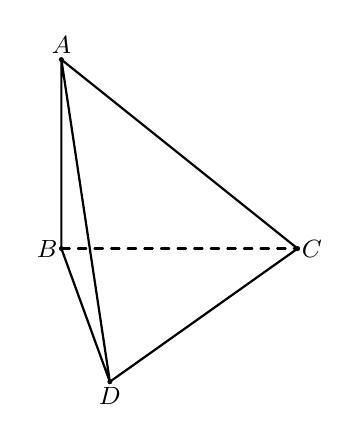
\begin{tikzpicture}[line join = round, line cap = round, thick, font = \small, scale = .6]
			\path
			(0:0) coordinate (B)
			+(0:5) coordinate (C)
			+(-70:3) coordinate (D)
			++(90:4) coordinate (A)
			;
			\draw[dashed]
			(B)--(C)
			;
			\draw
			(A)--(B)--(D)--(C)--cycle
			(A)--(D)
			;
			\foreach \x/\g in {B/180,C/0,D/-90,A/90}
			\fill (\x) circle (1.5pt)
			+(\g:3mm) node {$\x$};
		\end{tikzpicture}
	}
	\loigiai{
	}
\end{ex}
%Câu 2
\begin{ex}
	\immini{
		Cho hình lăng trụ tam giác $ABC.A'B'C'$.Gọi $M$, $N$ lần lượt là trung điểm của $AB$, $AC$. Trong 4 vectơ $\vec{AB}$, $\vec{CB}$, $\vec{B'C'}$, $\vec{A'C'}$ vectơ  nào cùng hướng với vectơ $\vec{MN}$
		\choice
		{$\vec{AB}$}
		{$\vec{CB}$}
		{\True $\vec{B'C'}$}
		{$\vec{A'C'}$}
	}{\begin{tikzpicture}[line join = round, line cap = round, thick, font = \small, scale = .7]
			\path
			(0:0) coordinate (A)
			+(0:4) coordinate (C)
			+(-50:2) coordinate (B)
			+(75:3.5) coordinate (A')
			($(A')+(B)-(A)$) coordinate (B')
			($(A')+(C)-(A)$) coordinate (C')
			($(A)!.5!(B)$) coordinate (M)
			($(A)!.5!(C)$) coordinate (N)
			;
			\draw[dashed]
			(A)--(C) (M)--(N)
			;
			\draw
			(A)--(B)--(C)--(C')--(A')--cycle
			(B')--(A') (B')--(B) (B')--(C')
			;
			\foreach \x/\g in {A/180,B/-90,C/0,A'/-180,B'/70,C'/0,M/-135,N/-45}
			\fill (\x) circle (1.5pt)
			+(\g:3mm) node {$\x$};
		\end{tikzpicture}
	}
	\loigiai{
		Vì $MN$ là đường trung bình của tam giác $ABC$ nên $MN$ song song với $BC$. Mà tứ giác $BCC'B'$ là hình bình hành. Do đó $MN$ song song với $B'C'$. Vậy hai vectơ $\vec{MN}$ và $\vec{B'C'}$ cùng hướng.
	}
\end{ex}
%Câu 3
\begin{ex}
	\immini{
		Cho hình hộp $ABCD.A'B'C'D'$.Số các vectơ có điểm đầu, điểm cuối là các đỉnh của hình hộp và bằng vectơ $\vec{AB}$ là
		\choice
		{$1$}
		{$2$}
		{\True $3$}
		{$4$}
	}{ \begin{tikzpicture}[line join = round, line cap = round, thick, font = \small, scale = .7]
			\path
			(0:0) coordinate (D')
			+(75:3.5) coordinate (D)
			+(0:3) coordinate (C')
			+(40:2) coordinate (A')
			($(C')+(D)-(D')$) coordinate (C)
			($(D)+(A')-(D')$) coordinate (A)
			($(C')+(A')-(D')$) coordinate (B')
			($(C)+(A)-(D)$) coordinate (B)
			;
			\draw[dashed]
			(A')--(A) (A')--(B') (A')--(D')
			;
			\draw
			(A)--(B)--(B')--(C')--(D')--(D)--cycle
			(C)--(B) (C)--(D) (C)--(C')
			;
			\foreach \x/\g in {D'/-90,C'/-90,D/180,A'/135,C/-45,A/90,B'/0,B/90}
			\fill (\x) circle (1.5pt)
			+(\g:3mm) node {$\x$};
		\end{tikzpicture}
	}
	\loigiai{
		$\vec{AB}=\vec{DC}=\vec{D'C'}=\vec{A'B'}$
	}
\end{ex}
%Câu 4
\begin{ex}
	Cho hình hộp $ABCD.A'B'C'D'$. Trong các khẳng định dưới đây, đâu là khẳng định đúng?
	\choice
	{$\vec{AB}+\vec{AC}+\vec{AD}=\vec{AC'}$}
	{\True $\vec{AB}+\vec{AA'}+\vec{AD}=\vec{AC'}$}
	{$\vec{AB}+\vec{AA'}+\vec{AD}=\vec{AC}$}
	{$\vec{AB}+\vec{AA'}+\vec{AD}=\vec{0}$}
	\loigiai{
		Xét hình hộp $ABCD.A'B'C'D'$ ta có $\vec{AB}+\vec{AA'}+\vec{AD}=\vec{AC'}$
	}
\end{ex}
%Câu 5
\begin{ex}
	Trong không gian cho tam giác $ABC$ có $G$ là trọng tâm và điểm $M$ nằm ngoài mặt phẳng $(ABC)$. Khẳng định nào sau đây là đúng?
	\choice
	{$\vec{MA}+\vec{MB}+\vec{MC}=\vec{0}$}
	{$\vec{GA}+\vec{GB}+\vec{GC}=0$}
	{$\vec{MA}+\vec{MB}+\vec{MC}=\vec{MG}$}
	{\True $\vec{MA}+\vec{MB}+\vec{MC}=3\vec{MG}$}
	\loigiai{
		Vì $G$ là trọng tâm tam giác $ABC$ nên $\vec{MA}+\vec{MB}+\vec{MC}=3\vec{MG}$
	}
\end{ex}
%Câu 6
\begin{ex}
	Cho hình chóp đều $S.ABCD$ tất cả các cạnh bằng $2\sqrt{3}$. Tính độ dài vectơ  $\vec{u}=\vec{SA}-\vec{SC}$.
	\choice
	{$\sqrt{3}$}
	{$\sqrt{2}$}
	{\True $2\sqrt{6}$}
	{$2\sqrt{2}$}
	\loigiai{
		Ta có: $|\vec{u}| = |\vec{SA}-\vec{SC}| = |\vec{CA}| = AB\sqrt{2} =2\sqrt{6}$.
	}
\end{ex}
%Câu 7
\begin{ex}
	Cho tứ diện $ABCD$. Mệnh đề nào dưới đây là mệnh đề đúng?
	\choice
	{$\vec{BC}-\vec{BA}=\vec{DA}-\vec{DC}$}
	{$\vec{AC}-\vec{AD}=\vec{BD}-\vec{BC}$}
	{\True $\vec{AB}-\vec{AC}=\vec{DB}-\vec{DC}$}
	{$\vec{AB}-\vec{AD}=\vec{CD}-\vec{CB}$}
	\loigiai{
		Ta có: $\heva{& \vec{AB}-\vec{AC}=\vec{CB} \\& \vec{DB}-\vec{DC}=\vec{CB}}\Rightarrow \vec{AB}-\vec{AC}=\vec{DB}-\vec{DC}$.
	}
\end{ex}
%Câu 8
\begin{ex}
	Cho hình lăng trụ $ABC.A'B'C'$, $M$ là trung điểm của $BB'$. Đặt $\vec{CA}=\vec{a}$, $\vec{CB}=\vec{b}$, $\vec{AA'}=\vec{c}$. Khẳng định nào sau đây đúng?
	\choice
	{$\vec{AM}=\vec{b}+\vec{c}-\dfrac{1}{2}\vec{a}$}
	{$\vec{AM}=\vec{a}-\vec{c}+\dfrac{1}{2}\vec{b}$}
	{$\vec{AM}=\vec{a}+\vec{c}-\dfrac{1}{2}\vec{b}$}
	{\True $\vec{AM}=\vec{b}-\vec{a}+\dfrac{1}{2}\vec{c}$}
	\loigiai{
		\immini{
			Ta có: $\vec{AM}=\vec{AB}+\vec{BM}=\vec{CB}-\vec{CA}+\dfrac{1}{2}\vec{BB'}=\vec{CB}-\vec{CA}+\dfrac{1}{2}\vec{AA'}=\vec{b}-\vec{a}+\dfrac{1}{2}\vec{c}$
		}{\begin{tikzpicture}[line join = round, line cap = round, thick, font = \small, scale = .6]
				\path
				(0:0) coordinate (A)
				+(0:4) coordinate (C)
				+(-50:2) coordinate (B)
				+(75:4) coordinate (A')
				($(A')+(B)-(A)$) coordinate (B')
				($(A')+(C)-(A)$) coordinate (C')
				($(B)!.5!(B')$) coordinate (M)
				;
				\draw[dashed]
				(A)--(C)
				;
				\draw
				(A)--(B)--(C)--(C')--(A')--cycle
				(B')--(A') (B')--(B) (B')--(C') (A)--(M)
				;
				\foreach \x/\g in {A/180,B/-90,C/0,A'/-180,B'/70,C'/0,M/135}
				\fill (\x) circle (1.5pt)
				+(\g:3mm) node {$\x$};
			\end{tikzpicture}
		}
	}
\end{ex}
%Câu 9
\begin{ex}
	Cho hình lập phương $ABCD.A'B'C'D'$ cạnh $a$. Tính độ dài véctơ $\vec{x}=\vec{A'C'}-\vec{A'A}$ theo $a$?
	\choice
	{$a\sqrt{2}$}
	{$\dfrac{a\sqrt{3}}{2}$}
	{$a\sqrt{6}$}
	{\True $a\sqrt{3}$}
	\loigiai{
		Ta có $\vec{x}=\vec{A'C'}-\vec{A'A}=\vec{AC'}=a\sqrt{3}$.
	}
\end{ex}
%Câu 10
\begin{ex}
	\immini{Cho tứ diện $S.ABC$ có $M$, $N$, $P$ là trung điểm của $SA$, $SB$, $SC$. Tìm khẳng định đúng?}
	{\begin{tikzpicture}[line join = round, line cap = round, thick, font = \small, scale = .7]
		\path 
		(0:0) coordinate (A)
		+(0:5) coordinate (C)
		+(-70:2) coordinate (B)
		+(65:4) coordinate (S)
		($(S)!.5!(A)$) coordinate (M)
		($(S)!.5!(B)$) coordinate (N)
		($(S)!.5!(C)$) coordinate (P)
		;
		\draw[dashed] 
		(A)--(C) (M)--(P)
		;
		\draw 
		(A)--(B)--(C)--(S)--cycle
		(S)--(B) (M)--(N)--(P)
		;
		\foreach \x/\g in {A/180,C/0,B/-90,S/45,M/135,N/-45,P/45}
		\fill (\x) circle (1.5pt)
		+(\g:3mm) node {$\x$};
		\end{tikzpicture}}
	\choice
	{$\vec{AB}=\dfrac{1}{2}\left(\vec{PN}-\vec{PM}\right)$}
	{$\vec{AB}=\vec{PN}-\vec{PM}$}
	{$\vec{AB}=2\left(\vec{PM}-\vec{PN}\right)$}
	{\True $\vec{AB}=2\left(\vec{PN}-\vec{PM}\right)$}
	\loigiai{
		Ta có: $\vec{AB}=2\vec{MN}=2\left(\vec{PN}-\vec{PM}\right)$.
	}
\end{ex}
%Câu 11
\begin{ex}
	\immini{Cho tứ diện $S.ABC$ có đáy là tam giác đều cạnh $a$, $SB$ vuông góc với đáy và $SB=\sqrt{3}a$. Góc giữa hai vectơ $(\vec{AB},\vec{AS})$ là}
	{\begin{tikzpicture}[line join = round, line cap = round, thick, font = \small, scale = .7]
		\path 
		(0:0) coordinate (B)
		+(0:5) coordinate (C)
		+(-50:3) coordinate (A)
		+(90:4) coordinate (S)
		;
		\draw[dashed] 
		(B)--(C)
		;
		\draw 
		(S)--(B)--(A)--(C)--cycle
		(S)--(A)
		\foreach \x/\y/\z in {S/B/C,S/B/A}{
		pic[draw, angle radius = 8pt]{right angle = \x--\y--\z}
		}
		;
		\foreach \x/\g in {B/180,C/0,A/-90,S/90}
		\fill (\x) circle (1.5pt)
		+(\g:3mm) node {$\x$};
		\end{tikzpicture}}
	\choice
	{\True $60^\circ$}
	{$30^\circ$}
	{$45^\circ$}
	{$90^\circ$}
	\loigiai{
		Ta có: $\left(\vec{AB},\vec{AS}\right)=\widehat{SAB}$.\\
		Xét $\triangle SBA$ vuông tại $B$ ta có: $\tan \left(\widehat{SAB}\right)=\dfrac{SB}{AB}=\sqrt{3}$. Suy ra: $\left(\vec{AB},\vec{AS}\right)=60^\circ$
	}
\end{ex}
%Câu 12
\begin{ex}
	Cho hình chóp $S.ABC$ có $AB=4$, $\widehat{BAC}=60^\circ$, $\vec{AB} \cdot \vec{AC}=6$. Khi đó độ dài $\vec{AC}$ là
	\choice
	{\True $3$}
	{$6$}
	{$4$}
	{$12$}
	\loigiai{
		Ta có: $\vec{AB} \cdot \vec{AC}=AB \cdot AC \cdot \cos \widehat{BAC}\Leftrightarrow 6=4 \cdot AC \cdot \cos 60^\circ \Leftrightarrow AC=3$.
	}
\end{ex}

\textbf{PHẦN II.Câu trắc nghiệm đúng sai. Trong mỗi ý a), b), c), d) ở mỗi câu, học sinh chọn đúng hoặc sai.}
%Câu 13
\begin{ex}
	\immini{Cho tứ diện $ABCD$ có $AB=AC=AD=a$ và $\widehat{BAC}=\widehat{BAD}=60^\circ ,\widehat{CAD}=90^\circ $. Gọi $I$ là điểm trên cạnh $AB$ sao cho $AI=3IB$ và $J$ là trung điểm của $CD$. Gọi $\alpha $ là góc giữa hai vectơ  $\vec{AB}$ và $\vec{IJ}$.
	\choiceTF
	{\True Tam giác $BCD$ vuông cân}
	{$\vec{IJ}=\dfrac{1}{2}\vec{AC}+\dfrac{1}{2}\vec{AD}+\dfrac{3}{2}\vec{AB}$}
	{$\vec{AB} \cdot \vec{AC}+\vec{AC} \cdot \vec{AD}+\vec{AD} \cdot \vec{AB}=\dfrac{a^2}{2}$}
	{\True $\cos \alpha =-\dfrac{\sqrt{5}}{5}$}
	}{\begin{tikzpicture}[line join = round, line cap = round, thick, font = \small, scale = .7]
		\path 
		(0:0) coordinate (B)
		+(0:5) coordinate (C)
		+(-70:2) coordinate (D)
		+(75:4) coordinate (A)
		($(B)!1/4!(A)$) coordinate (I)
		($(C)!.5!(D)$) coordinate (J)
		;
		\draw[dashed] 
		(B)--(C) (I)--(J)
		;
		\draw 
		(A)--(B)--(D)--(C)--cycle
		(A)--(D)
		;
		\foreach \x/\g in {B/180,C/0,D/-90,A/90,I/135,J/-45}
		\fill (\x) circle (1.5pt)
		+(\g:3mm) node {$\x$};
		\end{tikzpicture}}
	\loigiai{
		\begin{enumerate}[a)]
			\item Tam giác $ABC$, $ABD$ đều cạnh bằng $a$, tam giác $ACD$ vuông cân đỉnh $A\Rightarrow CD=a\sqrt{2}$. Vậy tam giác $BCD$ có $BC=BD=a,CD=a\sqrt{2}$ nên tam giác $BCD$ vuông cân.
			\item $\vec{IJ}=\vec{IA}+\vec{AJ}=-\dfrac{3}{4}\vec{AB}+\dfrac{1}{2}\left(\vec{AC}+\vec{AD}\right)=\dfrac{1}{2}\vec{AC}+\dfrac{1}{2}\vec{AD}-\dfrac{3}{4>}\vec{AB}$.
			\item Ta có: $\vec{AC} \cdot \vec{AD}=0$, $\vec{AB} \cdot \vec{AD}=AB \cdot AD \cdot \cos 60^\circ =\dfrac{a^2}{2}$, $\vec{AC} \cdot \vec{AB}=\dfrac{a^2}{2}$. Suy ra $\vec{AB} \cdot \vec{AC}+\vec{AC} \cdot \vec{AD}+\vec{AD} \cdot \vec{AB}=a^2$.\\
			\item $IJ^2=\vec{IJ}^2=\dfrac{1}{4}{{\left(\vec{AC}+\vec{AD}-\dfrac{3}{2}\vec{AB}\right)}^2}
				      =\dfrac{1}{4}\left(\dfrac{17}{4}a^2+2\vec{AC} \cdot \vec{AD}-3\vec{AC} \cdot \vec{AB}-3\vec{AB} \cdot \vec{AD}\right)
				      =\dfrac{5a^2}{16}\Rightarrow IJ=\dfrac{a\sqrt{5}}{4}$.\\
			      $\vec{IJ} \cdot \vec{AB}=\dfrac{1}{2}\left(\vec{AC}+\vec{AD}-\dfrac{3}{2}\vec{AB}\right) \cdot \vec{AB}= \dfrac{1}{2}\left(\vec{AC} \cdot \vec{AB}+\vec{AD} \cdot \vec{AB}-\dfrac{3}{2}{{\vec{AB}}^2}\right)=-\dfrac{a^2}{4}$.\\
			      $\cos \left(\vec{IJ},\vec{AB}\right)=\dfrac{\vec{IJ} \cdot \vec{AB}}{IJ \cdot AB}=\dfrac{-\dfrac{a^2}{4}}{\dfrac{a\sqrt{5}}{4} \cdot a}=-\dfrac{\sqrt{5}}{5}$.
		\end{enumerate}
	}
\end{ex}
%Câu 14
\begin{ex}
	\immini{Cho tứ diện $ABCD$. Gọi $M$, $N$, $P$, $Q$, $R$, $S$, $G$ lần lượt là trung điểm các đoạn thẳng $AB$, $CD$, $AC$, $BD$, $AD$, $BC$, $MN$.
	\choiceTF
	{\True $\vec{MR}=\vec{SN}$}
	{\True $\vec{GA}+\vec{GB}+\vec{GC}+\vec{GD}=\vec{0}$}
	{$2\vec{PQ}=\vec{AB}+\vec{AC}+\vec{AD}$}
	{\True $\vec{IA}+\vec{IB}+\vec{IC}+\vec{ID}|$ nhỏ nhất khi và chỉ khi điểm $I$ trùng với điểm $G$}
	}{\begin{tikzpicture}[line join = round, line cap = round, thick, font = \small, scale = .7]
		\path 
		(0:0) coordinate (B)
		+(0:5) coordinate (C)
		+(-70:2) coordinate (D)
		+(75:4) coordinate (A)
		($(A)!.5!(B)$) coordinate (M)
		($(C)!.5!(D)$) coordinate (N)
		($(A)!.5!(C)$) coordinate (P)
		($(B)!.5!(D)$) coordinate (Q)
		($(A)!.5!(D)$) coordinate (R)
		($(B)!.5!(C)$) coordinate (S)
		($(M)!.5!(N)$) coordinate (G)
		;
		\draw[dashed] 
		(B)--(C) (M)--(N)
		;
		\draw 
		(A)--(B)--(D)--(C)--cycle
		(A)--(D)
		;
		\foreach \x/\g in {B/180,C/0,D/-90,A/90,M/135,N/-45,P/45,Q/-135,R/180,S/45,G/45}
		\fill (\x) circle (1.5pt)
		+(\g:3mm) node {$\x$};
		\end{tikzpicture}}
	\loigiai{
		\begin{center}
			\begin{tikzpicture}[line join = round, line cap = round, thick, font = \small, scale = .7]
				\path 
				(0:0) coordinate (B)
				+(0:5) coordinate (C)
				+(-70:2) coordinate (D)
				+(75:4) coordinate (A)
				($(A)!.5!(B)$) coordinate (M)
				($(C)!.5!(D)$) coordinate (N)
				($(A)!.5!(C)$) coordinate (P)
				($(B)!.5!(D)$) coordinate (Q)
				($(A)!.5!(D)$) coordinate (R)
				($(B)!.5!(C)$) coordinate (S)
				($(M)!.5!(N)$) coordinate (G)
				;
				\draw[dashed] 
				(B)--(C) (M)--(N) (P)--(Q) (R)--(S)
				;
				\draw 
				(A)--(B)--(D)--(C)--cycle
				(A)--(D)
				;
				\foreach \x/\g in {B/180,C/0,D/-90,A/90,M/135,N/-45,P/45,Q/-135,R/180,S/45,G/45}
				\fill (\x) circle (1.5pt)
				+(\g:3mm) node {$\x$};
				\end{tikzpicture}
		\end{center}
		\begin{enumerate}[a)]
			\item $\vec{MR}=\vec{SN}=\dfrac12 \vec{BD}$.
			\item Vì $M$ là trung điểm của $AB$ nên $\vec{GA}+\vec{GB}=2\vec{GM}$\\
			      Vì $N$ là trung điểm của $CD$ nên $\vec{GC}+\vec{GD}=2\vec{GN}$\\
			      Vì $G$ là trung điểm của $MN$ nên $\vec{GM}+\vec{GN}=\vec{0}$\\
			      Do đó: $\vec{GA}+\vec{GB}+\vec{GC}+\vec{GD}=2\left(\vec{GM}+\vec{GN}\right)=2 \cdot \vec{0}=\vec{0}$.
			\item $\vec{PQ}=\vec{AQ}-\vec{AP}=\dfrac{1}{2}\left(\vec{AB}+\vec{AD}\right)-\dfrac{1}{2}\vec{AC}\Leftrightarrow 2\vec{PQ}=\vec{AB}-\vec{AC}+\vec{AD}$
			\item $\vec{IA}+\vec{IB}+\vec{IC}+\vec{ID}=4\vec{IG}+\left(\vec{GA}+\vec{GB}+\vec{GC}+\vec{GD}\right)=4\vec{IG}$.\\
			      $\Rightarrow | \vec{IA}+\vec{IB}+\vec{IC}+\vec{ID}|=| 4\vec{IG}|=4IG$\\
			      Do đó: $| \vec{IA}+\vec{IB}+\vec{IC}+\vec{ID}|$ nhỏ nhất khi $IG=0\Leftrightarrow I\equiv G$
		\end{enumerate}
	}
\end{ex}
%Câu 15
\begin{ex}
	\immini{Cho hình hộp chữ nhật $ABCD \cdot EFGH$ có $AB=AE=2$, $AD=3$ và đặt $\vec{a}=\vec{AB},\vec{b}=\vec{AD},\vec{c}=\vec{AE}$. Lấy điểm $M$ thỏa $\vec{AM}=\dfrac{1}{5}\vec{AD}$ và điểm $N$ thỏa $\vec{EN}=\dfrac{2}{5}\vec{EC}$. (tham khảo hình vẽ).
	\choiceTF
	{\True $\vec{MA}=-\dfrac{1}{5}\vec{b}$}
	{\True $\vec{EN}=\dfrac{2}{5}\left(\vec{a}-\vec{b}+\vec{c}\right)$}
	{${{\left(m \cdot \vec{a}+n \cdot \vec{b}+n \cdot \vec{c}\right)}^2}=m^2 \cdot {{\vec{a}}^2}+n^2 \cdot {{\vec{b}}^2}+p^2 \cdot {{\vec{c}}^2}$ với $m,n,p$ là các số thực}
	{\True $MN=\dfrac{\sqrt{61}}{5}$}
	}{\begin{tikzpicture}[line join = round, line cap = round, thick, font = \small, scale = .7]
		\path
		(0:0) coordinate (H)
		+(75:3.5) coordinate (D)
		+(0:3) coordinate (G)
		+(40:2) coordinate (E)
		($(G)+(D)-(H)$) coordinate (C)
		($(D)+(E)-(H)$) coordinate (A)
		($(G)+(E)-(H)$) coordinate (F)
		($(C)+(A)-(D)$) coordinate (B)
		;
		\draw[dashed]
		(E)--(A) (E)--(F) (E)--(H)
		;
		\draw
		(A)--(B)--(F)--(G)--(H)--(D)--cycle
		(C)--(B) (C)--(D) (C)--(G)
		;
		\foreach \x/\g in {H/-90,G/-90,D/180,E/135,C/-45,A/90,F/0,B/90}
		\fill (\x) circle (1.5pt)
		+(\g:3mm) node {$\x$};
	\end{tikzpicture}}
	\loigiai{
		\begin{enumerate}[a)]
			\item $\vec{MA}=-\vec{AM}=-\dfrac{1}{5}\vec{AD}=-\dfrac{1}{5}\vec{b}$.
			\item $\vec{EN}=\dfrac{2}{5}\vec{EC}=\dfrac{2}{5}\left(\vec{EF}+\vec{EH}+\vec{EA}\right)=\dfrac{2}{5}\left(\vec{a}+\vec{b}-\vec{c}\right)$.
			\item ${{\left(m \cdot \vec{a}+n \cdot \vec{b}+p \cdot \vec{c}\right)}^2}=m^2 \cdot {{\vec{a}}^2}+n^2 \cdot {{\vec{b}}^2}+p^2 \cdot {{\vec{c}}^2}+2mn \cdot \vec{a} \cdot \vec{b}+2np \cdot \vec{b} \cdot \vec{c}+2mp \cdot \vec{a} \cdot \vec{c}$\\
			      $=m^2 \cdot {{\vec{a}}^2}+n^2 \cdot {{\vec{b}}^2}+p^2 \cdot {{\vec{c}}^2}$. (vì $\vec{a},\vec{b},\vec{c}$ đôi một vuông góc nên $\vec{a} \cdot \vec{b}=\vec{b} \cdot \vec{c}=\vec{a} \cdot \vec{c}=0$).
			\item $\vec{MN}=\vec{MA}+\vec{AE}+\vec{EN}=-\dfrac{1}{5}\vec{b}+\vec{c}+\dfrac{2}{5}\left(\vec{a}+\vec{b}-\vec{c}\right)=\dfrac{2}{5}\vec{a}+\dfrac{1}{5}\vec{b}+\dfrac{3}{5}\vec{c}$.\\
			      $MN^2={{\vec{MN}}^2}={{\left(\dfrac{2}{5}\vec{a}+\dfrac{1}{5}\vec{b}+\dfrac{3}{5}\vec{c}\right)}^2}=\dfrac{4}{25}{{\vec{a}}^2}+\dfrac{1}{25}{{\vec{b}}^2}+\dfrac{9}{25}{{\vec{c}}^2}=\dfrac{4}{25} \cdot 4+\dfrac{1}{25} \cdot 9+\dfrac{9}{25} \cdot 4=\dfrac{61}{25}$.\\
			      Suy ra $MN=\dfrac{\sqrt{61}}{5}$.
		\end{enumerate}
	}
\end{ex}
%Câu 16
\begin{ex}
	\immini{Cho hình lăng trụ tam giác đều $ABC.A'B'C'$ có cạnh đáy bằng $x$ và chiều cao bằng $y$. (tham khảo hình vẽ)
	\choiceTF
	{\True $\vec{AB} \cdot \vec{AC}=\dfrac{1}{2}x^2$}
	{\True $\vec{AC'}=\vec{AC}+\vec{AA'}$}
	{$\vec{CB'}=\vec{AB}-\vec{CA}+\vec{AA'}$}
	{Góc $\left(AC',CB'\right)>60^\circ $ khi $\dfrac{y}{x}<\sqrt{2}$}
	}{\begin{tikzpicture}[line join = round, line cap = round, thick, font = \small, scale = .6]
		\path
		(0:0) coordinate (A)
		+(0:4) coordinate (C)
		+(-50:2) coordinate (B)
		+(90:4) coordinate (A')
		($(A')+(B)-(A)$) coordinate (B')
		($(A')+(C)-(A)$) coordinate (C')
		;
		\draw[dashed]
		(A)--(C)
		;
		\draw
		(A)--(B)--(C)--(C')--(A')--cycle
		(B')--(A') (B')--(B) (B')--(C')
		;
		\foreach \x/\g in {A/180,B/-90,C/0,A'/-180,B'/70,C'/0}
		\fill (\x) circle (1.5pt)
		+(\g:3mm) node {$\x$};
	\end{tikzpicture}}
	\loigiai{
		\begin{enumerate}[a)]
			\item $\vec{AB} \cdot \vec{AC}=AB \cdot AC \cdot \cos 60^\circ =\dfrac{1}{2}x^2$.
			\item $\vec{AC'}=\vec{AC}+\vec{AA'}$ (vì $ACC'A'$ là hình chữ nhật).
			\item $\vec{CB'}=\vec{CB}+\vec{CC'}=\vec{AB}-\vec{AC}+\vec{AA'}$.
			\item Ta có $\vec{AC'} \cdot \vec{CB'}=\left(\vec{AC}+\vec{AA'}\right) \cdot \left(\vec{AB}-\vec{AC}+\vec{AA'}\right)=y^2-\dfrac{1}{2}x^2$ và $AC'=CB'=\sqrt{x^2+y^2}$.\\
			      Khi đó $\cos \left(AC',CB'\right)=\left| \cos \left(\vec{AC'},\vec{CB'}\right) \right|=\dfrac{\left| \vec{AC'} \cdot \vec{CB'} \right|}{AC' \cdot CB'}=\dfrac{\left| y^2-\dfrac{1}{2}x^2\right|}{x^2+y^2}$.\\
			      Theo đề $\left(AC',CB'\right)>60^\circ $, suy ra $\dfrac{\left| y^2-\dfrac{1}{2}x^2\right|}{x^2+y^2}<\dfrac{1}{2}\Leftrightarrow 3y^4-6x^2y^2<0\Leftrightarrow \dfrac{y}{x}<\sqrt{2}$.
		\end{enumerate}
	}
\end{ex}
PHẦN III. Câu trắc nghiệm trả lời ngắn. Thí sinh trả lời từ câu 1 đến câu 6
%Câu 17
\begin{ex}
	\immini{Cho hình lăng trụ $ABC.A'B'C'$. Đặt $\vec{AB}=\vec{a},\vec{AA'}=\vec{b},\vec{AC}=\vec{c}$. Ta biểu diễn $\vec{B'C}=m\vec{a}+n\vec{b}+p\vec{c}$, khi đó $m+n+p$ bằng bao nhiêu?}
	{\begin{tikzpicture}[line join = round, line cap = round, thick, font = \small, scale = .6]
		\path
		(0:0) coordinate (A)
		+(0:4) coordinate (C)
		+(-50:2) coordinate (B)
		+(75:4) coordinate (A')
		($(A')+(B)-(A)$) coordinate (B')
		($(A')+(C)-(A)$) coordinate (C')
		;
		\draw[dashed]
		(A)--(C)
		;
		\draw
		(A)--(B)--(C)--(C')--(A')--cycle
		(B')--(A') (B')--(B) (B')--(C')
		;
		\foreach \x/\g in {A/180,B/-90,C/0,A'/-180,B'/70,C'/0}
		\fill (\x) circle (1.5pt)
		+(\g:3mm) node {$\x$};
	\end{tikzpicture}}
	\loigiai{
		\SA{-1}
		$\vec{B'C}=\vec{B'B}+\vec{BC}=-\vec{BB'}+\vec{BA}+\vec{AC}=-\vec{BB'}-\vec{AB}+\vec{AC}=-\vec{b}-\vec{a}+\vec{c}$\\
		$\Rightarrow \vec{B'C}=-\vec{a}-\vec{b}+\vec{c}$.\\
		Suy ra $m=-1$, $n=-1$, $p=1$. Do đó $m+n+p=-1$.
	}
\end{ex}
%Câu 18
\begin{ex}
	Cho tứ diện $ABCD$, gọi $I$, $J$ lần lượt là trung điểm của $AB$ và $CD$. Biết $\vec{IJ}=\dfrac{a}{b}\vec{AC}+\dfrac{c}{d}\vec{BD}$. Giá trị biểu thức $P=ab+cd$ bằng
	\loigiai{
		\SA{4}
		$\vec{AC}+\vec{BD}=\vec{AI}+\vec{IJ}+\vec{JC}+\vec{BI}+\vec{IJ}+\vec{JD}=2\vec{IJ}\Rightarrow \vec{IJ}=\dfrac{1}{2}\left(\vec{AC}+\vec{BD}\right)$.
	}
\end{ex}
%Câu 19
\begin{ex}
	Cho tứ diện đều $ABCD$ có cạnh bằng $4$. Giá trị tích vô hướng $\vec{AB}\left(\vec{AB}-\vec{CA}\right)$ bằng
	\loigiai{
		\SA{24}
		$\begin{aligned}[t]
				\vec{AB}\left(\vec{AB}-\vec{CA}\right)
				 & =\vec{AB} \cdot \vec{AB}+\vec{AB} \cdot \vec{AC}={{\vec{AB}}^2}+| \vec{AB}| \cdot | \vec{AC}| \cdot \cos \left(\vec{AB},\vec{AC}\right)     \\
				 & =AB^2+AB \cdot AC \cdot \cos \left(\widehat{BAC}\right)=4^2+4 \cdot 4 \cdot \cos 60^\circ=4^2+\dfrac{4^2}{2}=\dfrac{{{3 \cdot 4}^2}}{2}=24.
			\end{aligned}$
	}
\end{ex}
%Câu 20
\begin{ex}
	Trong không gian, cho hai vectơ  $\vec{a}$ và $\vec{b}$ có cùng độ dài bằng $6$. Biết độ dài của vectơ  $\vec{a}+2\vec{b}$ bằng $6\sqrt{3}$. Biết số đo góc giữa hai vectơ  $\vec{a}$ và $\vec{b}$ là $x$ độ. Giá trị của $x$ là bao nhiêu?
	\loigiai{
		\SA{120}
		$\vec{a} \cdot \vec{b} = \dfrac{1}{4} \left[\left(\vec{a}+2 \vec{b}\right)^2 - \vec{a}^2 - 4\vec{b}^2\right]
			= \dfrac{1}{4} \left[\left|\vec{a}+2 \vec{b}\right|^2 - |\vec{a}|^2 - 4|\vec{b}|^2\right]
			= \dfrac{1}{4} \left[\left(6\sqrt{3}\right)^2 - 6^2 - 4\cdot 6^2\right] = -18$.\\
		Lại có $\vec{a} \cdot \vec{b}=| \vec{a}| \cdot | \vec{b}| \cdot \cos \left(\vec{a}\,,\vec{b}\right)\Leftrightarrow \cos \left(\vec{a}\,,\vec{b}\right)=\dfrac{\vec{a} \cdot \vec{b}}{| \vec{a}| \cdot | \vec{b}|}=\dfrac{-18}{6 \cdot 6}=\dfrac{-1}{2}\Leftrightarrow \left(\vec{a}\,,\vec{b}\right)=120^\circ $.\\
		Khi đó góc giữa hai vectơ  $\vec{a}$ và $\vec{b}$ là $120^\circ $.
	}
\end{ex}
%Câu 21
\begin{ex}
	Cho tứ diện đều $ABCD$ có cạnh bằng $15$. Biết độ dài của $\vec{AB}+\vec{AC}+\vec{AD}$ bằng $a\sqrt{6}$, khi đó giá trị của $a$ là?
	\loigiai{
	\SA{15}
	\immini{
	Gọi $G$ là trọng tâm tâm giác $BCD$, $M$ là trung điểm $CD$.\\
	Ta có $\vec{GB}+\vec{GC}+\vec{GD}=\vec{0}\Leftrightarrow \left(\vec{GA}+\vec{AB}\right)+\left(\vec{GA}+\vec{AC}\right)+\left(\vec{GA}+\vec{AD}\right)=\vec{0}\Leftrightarrow 3\vec{GA}+\left(\vec{AB}+\vec{AC}+\vec{AD}\right)=\vec{0}$\\
	$\Leftrightarrow \vec{AB}+\vec{AC}+\vec{AD}=-3\vec{GA}=3\vec{AG}\Rightarrow | \vec{AB}+\vec{AC}+\vec{AD}|=| 3\vec{AG}|=3AG$.\\
	Xét tam giác đều $BCD$ có $BM=BC \cdot \dfrac{\sqrt{3}}{2}=\dfrac{15\sqrt{3}}{2}\Rightarrow BG=\dfrac{2}{3}BM=5\sqrt{3}$.\\
	Vì tứ diện $ABCD$ đều nên $AG\bot (BCD)\Rightarrow \widehat{AGB}=90^\circ $.\\
	Xét tam giác $ABG$ có $AG=\sqrt{AB^2-BG^2}=\sqrt{{{15}^2}-{{\left(5\sqrt{3}\right)}^2}}=5\sqrt{6}$.\\
	Do đó $| \vec{AB}+\vec{AC}+\vec{AD}|=3AG=15\sqrt{6}\Rightarrow a=15$.\\
	Vậy giá trị của $a=15$.
	}{\begin{tikzpicture}[line join = round, line cap = round, thick, font = \small, scale = .7]
		\path 
		(0:0) coordinate (B)
		+(0:5) coordinate (C)
		+(-70:3) coordinate (D)
		(barycentric cs:B=1,C=1,D=1) coordinate (G)
		++(90:4) coordinate (A)
		($(C)!.5!(D)$) coordinate (M)
		;
		\draw[dashed] 
		(M)--(B)--(C) (A)--(G) 
		;
		\draw 
		(A)--(B)--(D)--(C)--cycle
		(A)--(D)
		;
		\foreach \x/\g in {B/180,C/0,D/-90,G/45,A/90,M/-45}
		\fill (\x) circle (1.5pt)
		+(\g:3mm) node {$\x$};
		\end{tikzpicture}}
	}
\end{ex}
%Câu 22
\begin{ex}
	Một chiếc cân đòn tay đang cân một vật có khối lượng $m=3\,\text{kg}$ được thiết kế với đĩa cân được giữ bởi bốn đoạn xích $SA$, $SB$, $SC$, $SD$ sao cho $S.ABCD$ là hình chóp tứ giác đều có $\widehat{ASC}=90^\circ $. Biết độ lớn của lực căng cho mỗi sợi xích có dạng $\dfrac{a\sqrt{2}}{4}$. Lấy $g=10 \mathrm{m}/\mathrm{s}^2$, khi đó giá trị của $a$ bằng bao nhiêu?
	\begin{center}
		\includegraphics{datak40/2D2-1/candon.png}
	\end{center}
	\loigiai{
		\SA{30}
		\immini{
		Gọi $O$ là tâm của hình vuông $ABCD$.\\
		Ta có $\vec{OA}+\vec{OB}+\vec{OC}+\vec{OD}=\vec{0}\Leftrightarrow \vec{OS}+\vec{SA}+\vec{OS}+\vec{SB}+\vec{OS}+\vec{SC}+\vec{OS}+\vec{SD}=\vec{0}$\\
		$\Leftrightarrow \vec{SA}+\vec{SB}+\vec{SC}+\vec{SD}=-4\vec{OS}=4\vec{SO}\Rightarrow | \vec{SA}+\vec{SB}+\vec{SC}+\vec{SD}| =| 4\vec{SO}|=4SO$.\\
		Trọng lượng của vật nặng là $P=mg=3 \cdot 10=30$ (N). Suy ra $4| \vec{SO}|=P=30$ (N) $\Rightarrow SO=\dfrac{15}{2}$.\\
		Lại có tam giác $ASC$ vuông cân tại $S$ nên\\
		$SO=SA \cdot \sin \widehat{SAC}\Rightarrow SA=\dfrac{SO}{\sin \widehat{SAC}}=\dfrac{\dfrac{15}{2}}{\sin 45^\circ }=\dfrac{15\sqrt{2}}{2}=\dfrac{30\sqrt{2}}{4}\Rightarrow a=30$.\\
		Vậy $a=30$.
		}{\begin{tikzpicture}[line join = round, line cap = round, thick, font = \small, scale = .7]
			\path 
			(0:0) coordinate (A)
			+(0:5) coordinate (B)
			+(-140:2.5) coordinate (D)
			($(B)+(D)-(A)$) coordinate (C)
			(intersection of A--C and B--D) coordinate (O)
			++(90:5) coordinate (S)
			;
			\draw[dashed] 
			(A)--(B) (A)--(D) (A)--(S) (A)--(C) (B)--(D) (S)--(O)
			;
			\draw 
			(D)--(C)--(B)
			(S)--(B) (S)--(C) (S)--(D)
			;
			\foreach \x/\g in {A/135,B/0,C/-45,D/-135,O/-90,S/90}
			\fill (\x) circle (1.5pt)
			+(\g:3mm) node {$\x$};
			\end{tikzpicture}}
	}
\end{ex}
